\chapter{Ontology-driven web system}
\label{cha:trafficDangerWebSystem}

\section{Introduction}
\label{sec:introductionTochapter4}

As it was mentioned at the beginning of the thesis, the system creation aim is an attempt to integrate database and ontology approach, for storing and inferring desired information about some domain in real time. In this chapter, such a composite approach is presented, in which location details of traffic conditions are stored in database, while clean abstract of traffic danger concept is described by core ontology. Such an integration results in dynamic deduction possibility of desired knowledge, using the ontology-based approach, instead of using static relations defined in database only.

The program cooperates with traffic danger ontology, and synchronizes that ontology with information stored in database. Next part of the process is traffic dangers inference. In this part reasoner searches for dangers, which occur on selected locations. Traffic dangers fetch the criteria only, when potentially dangerous traffic conditions are localized on area, we are looking for dangers. Locations of traffic conditions occurrences are defined by postal codes. In database, postal codes are connected with streets. Streets in turn are connected with districts. Ontology describes the way of connections between mentioned locations. Because of that fact, ontology gives the possibility of answering, which kind of traffic danger can occur on the desired location (postal code, street or district). As it was said before, the deduction is based on specific traffic conditions connected to specific postal codes.

Users are allowed to create dynamic questions, and getting results of inferred traffic dangers. That functionality is provided by the front dashboard page. Additionally, system allows trusted users to make changes to locations of traffic conditions occurrence. For working with latest data, provided by trusted users, synchronization mechanism is implemented. Synchronization integrates core ontology, describing the abstract of traffic dangers, with specific real time data. Synchronization process is executed first time on application startup. The startup can be understand as first request to the server while accessing main page. That functionality is also available on demand, after pressing synchronization button. After synchronization, we are cooperating with ontology cached in memory.

The project is coded in Java. Dependencies management and versioning is the task of Apache Maven tool. Main technologies used inside are: PostgreSQL, Hibernate, JSP, Spring MVC, jQuery, The OWL API, HermiT and Log4j.

\section{Ontology-driven software development}
\label{sec:ontologyDrivenSoftwareDevelopment}

An important aspect in developing any Semantic Web application, including application described in that chapter, is the ontology-driven architecture. In a simplification ontology-driven concept is extracted below:

\medskip

\begin{figure}[htp]
\centering
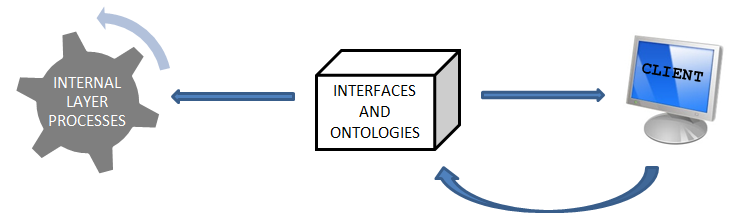
\includegraphics[scale=0.5]{images/chapter4/OntologyDrivenConcept}
\caption{Ontology-driven approach}
\label{fig:ontologyDrivenConcept}
\end{figure}

\noindent We can see that Semantic Web application in general is divided into 2 separate but linked layers \cite{OntDrivDev}:
\begin{itemize}
    \setlength{\itemsep}{0cm}
    \setlength{\parskip}{0cm}

    \item internal layer - contains all software logic: storage, control and deduction processes,
    \item Semantic Web layer - makes ontologies and interfaces available to the public.
\end{itemize}

\noindent Semantic Web layer is the external part. Interfaces of that layer are used to control the internal behavior, in particular the outcome of reasoning algorithms. Because of reusability of the ontologies, it is required to spend relatively lot of effort to provide good design and tests of that part. Domain experts should be involved in developing these tasks in parallel with programmers, to provide short iterations in developing as a results of quick responses for every inconsistencies in ontology like irrelevant hidden relationships, domain descriptions mistakes or usability problems. 

\subsection{Agile methodology}
\label{sub:agileMethodology}

All of that suggests, that software development based on agile methodologies is going to be the very dedicated while working on Semantic Web systems. Agile software development is based on iterative development, where requirements and solutions evolve through collaboration between self-organizing cross-functional teams. The term was introduced in the Agile Manifesto in 2001, which says:

\newpage

\noindent \textit{"We are uncovering better ways of developing software by doing it and helping others do it. Through this work we have come to value:}

\begin{itemize}
    \setlength{\itemsep}{0cm}
    \setlength{\parskip}{0cm}

    \item[] \textit{\textbf{individuals and interactions} over processes and tools,}
    \item[] \textit{\textbf{working software} over comprehensive documentation,}
    \item[] \textit{\textbf{customer collaboration} over contract negotiation,}
    \item[] \textit{\textbf{responding to change} over following a plan.}
\end{itemize}

\noindent \textit{That is, while there is value in the items on the right, we value the items on the left more"} \cite{AgileManifesto}.

\subsection{Model-driven architecture}
\label{sub:modelDrivenArchitecture}

Ontology-driven software design approach has a lot in common with model-driven architecture (MDA). MDA movement was launched by the Object Management Group (OMG) in 2001. That approach shows \textit{"how to better integrate high-level domain models into the development cycles of conventional software"} \cite{OntDrivDev}.

A central idea of MDA is to defines system functionality using a platform-independent model (PIM) using an appropriate domain-specific language (DSL). The PIM is next translated to one or more platform-specific models (PSMs) that computers can run. In the other words the goal of MDA is to employ languages like UML and generate from them a code appropriate for specific platform. Ontology-driven software development follows similar idea, but the way it does it is much more aggressive. It is because domain models can be used not only for code generation, but what is more remarkable, they can be involved in run time executable tasks. 

Nevertheless, any progress in MDA technology and tools may be useful for the Semantic Web community. In addition, MDA has aggregated wide range of modeling language standards under one metamodel writing standard called Meta-Object Facility (MOF). The OMG has created an initiative for rapid development ontology-related technologies. One of the OMG's efforts are directed towards mapping definition between OWL and MOF/UML. That integration can become a key for bringing that technologies much closer together. Because OWL does not need to be the best modeling language for everyone who is involved in domain design tasks, domain-specific languages can be used, depending on the task and
the expertise of the domain modelers. Platform dependent languages can be then translated into the details of OWL or any other desired language.

\newpage

\section{System use cases}
\label{sec:systemUseCases}

On the diagram below, actors and use cases of the system are shown:

\medskip

\begin{figure}[htp]
\centering
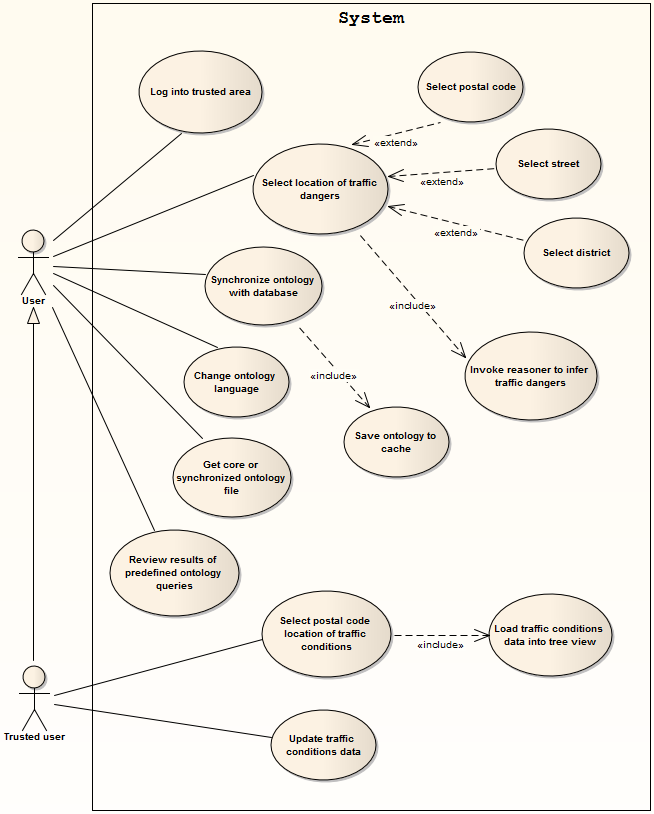
\includegraphics[scale=0.58]{images/chapter4/UseCase}
\caption{Use cases of the system}
\label{fig:useCases}
\end{figure}

\newpage

\section{Interaction with system for updating and inferring data}
\label{sec:interaction}

On the diagram below, sequence diagram for updating and inferring data is shown:

\medskip

\begin{figure}[htp]
\centering
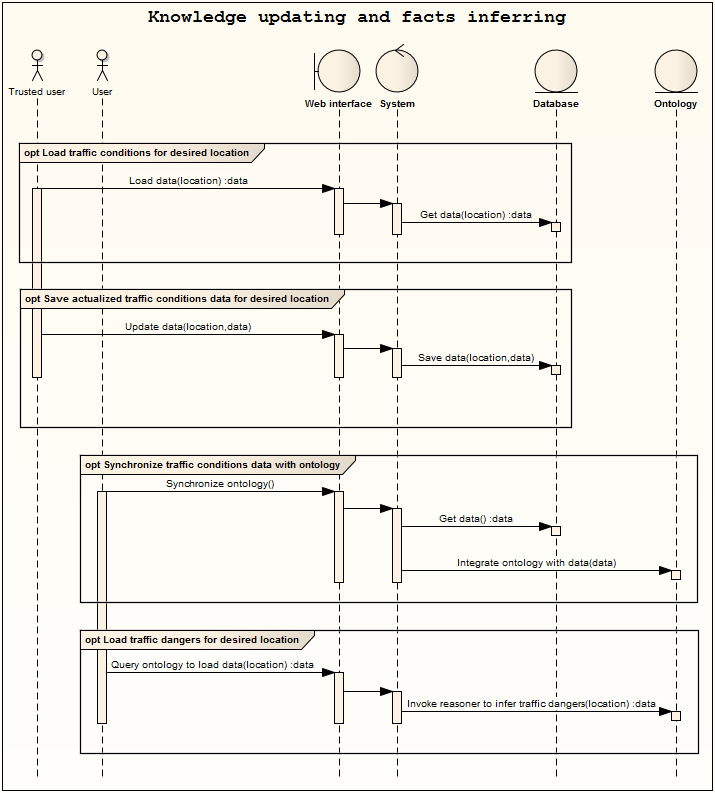
\includegraphics[scale=0.58]{images/chapter4/Sequence}
\caption{Sequence diagram for updating and inferring data}
\label{fig:sequence}
\end{figure}

\newpage

\section{System flow}
\label{sec:systemFlow}

On the diagram below, data flow in the system is shown:

\medskip

\begin{figure}[htp]
\centering
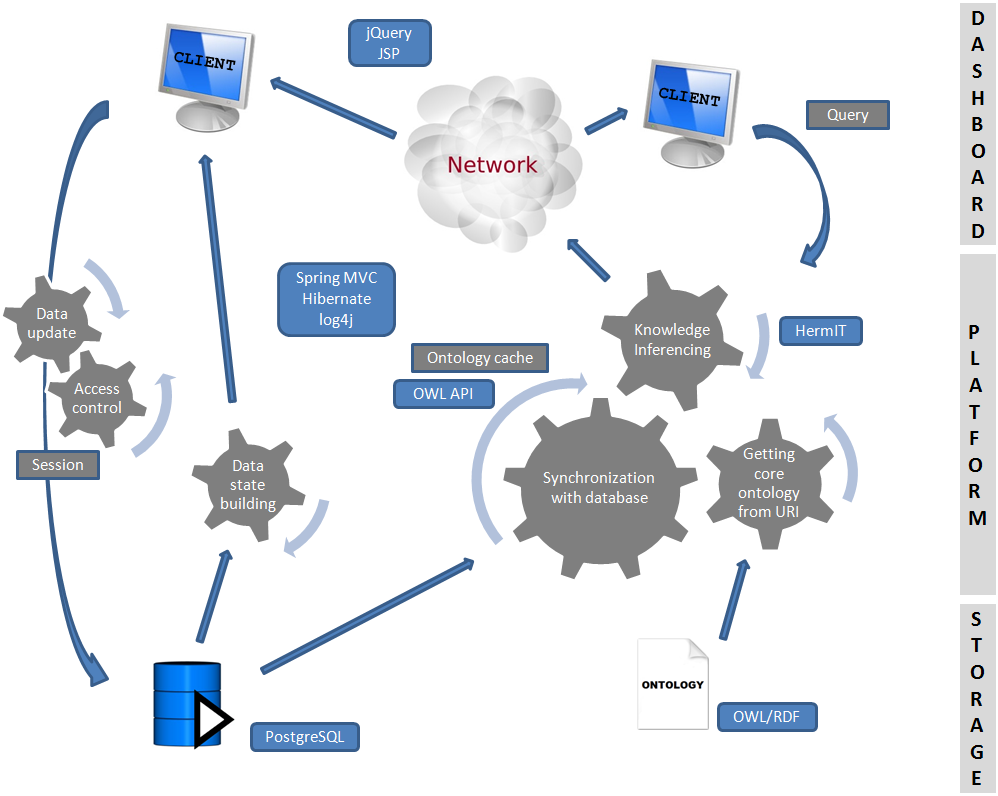
\includegraphics[scale=0.5]{images/chapter4/Flow}
\caption{Data flow in the system}
\label{fig:flow}
\end{figure}

\begin{tabular}[htb]{m{2cm}m{6cm}m{2cm}m{6cm}}
    
\includegraphics[scale=0.7]{images/chapter4/OperationIcon}      & Operation         & 
\includegraphics[scale=0.7]{images/chapter4/AnnotationIcon}       & Annotation \\
    
\includegraphics[scale=0.7]{images/chapter4/TechnologyIcon}     & Technology used   & 
\includegraphics[scale=0.7]{images/chapter4/SystemFlowIcon}       & Internal system flow \\
    
\includegraphics[scale=0.7]{images/chapter4/UserInputIcon}      & User input        & 
\includegraphics[scale=0.7]{images/chapter4/SystemPartNameIcon}   & System layer
\end{tabular}

\newpage

\noindent The system is divided into 3 functionally different layers: web dashboard layer cooperating with users (through browser clients), platform layer which is the core of system and storage layer, where data is stored, including ontology which drives the system. 

On the left part of the diagram we can see session established for trusted users (after authentication pass), who can modify system database data. Database data can be modified through assigning specified information to dynamically built tree of current data state. 

On the top, diagram shows, that all users can interact with dashboard for querying system, to get desired information. 

In the center of the figure there are 3 processes: downloading of the core ontology, synchronization core ontology with current data uploaded by trusted users and inferring ontology dependencies. Core ontology can be stored on local or remote server and is accessed by URI of location. Synchronization is based on OWL API library, and provides fresh information (cached in memory) for semantic reasoner to infer, as a response to end users queries. Deduction of classes is provided by HermiT reasoner. 

Cooperation with database is provided through Hibernate ORM technology. User interface is built with Java Server Pages and jQuery JavaScript library, while requests from users and appropriate responses, are controlled by Spring MVC. For logging the results of particular operations, Log4j library is used. Ontology can be provided in different formats like OWL2 XML, RDF/XML or Manchester Syntax. PostgreSQL is chosen as SQL database server. All of the mentioned technologies are free and open source.

\begin{framed}
\noindent It is just a brief preview of the system main tasks and particular technologies. The layers cooperation will be explained in detail in the next chapters. There will be also very short preview of mentioned technologies, which are used to build the project.
\end{framed}

\newpage

\section{Database structure}
\label{sec:databaseStructure}

Entity relationship diagram is shown in Figure \ref{fig:erd}. The diagram was made using Toad Data Modeler \cite{CasestudioHome}.

\medskip

\begin{figure}[htp]
\centering
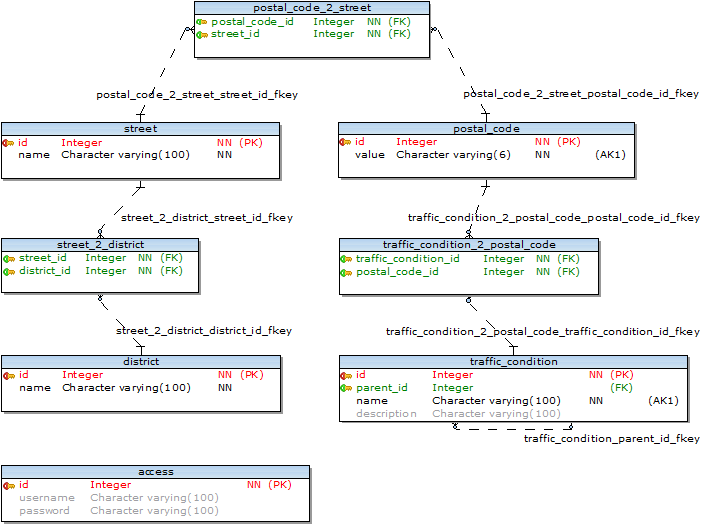
\includegraphics[scale=0.7]{images/chapter4/ERD}
\caption{ER diagram of \texttt{traffic} database}
\label{fig:erd}
\end{figure}

\noindent Database tables structure consist of tables describing locations: \texttt{street}, \texttt{district} and \texttt{postal\_code}, tables handling many-to-many relationships: \texttt{postal\_code\_2\_street}, \texttt{street\_2\_district}, \texttt{traffic\_condition\_2\_postal\_code}, table with traffic conditions structure \texttt{traffic\_condition} and table providing authentication for users: \texttt{access}.

\newpage

\begin{tabularx}{\textwidth}{X>{\hsize=10.5cm}X}
    \vtop{\vskip 0pt \vskip -\ht\strutbox 
    \begin{tabular}{|l|l|}
        \hline
        \multicolumn{2}{|c|}{\texttt{street}} \\
        \hline 
        \textcolor{blue}{\texttt{id}} & street unique identifier \\
        \textcolor{blue}{\texttt{name}} & street name \\
        \hline
    \end{tabular}
    \vskip -\dp\strutbox }%
    & Table contains streets names, used for defining locations of specific traffic conditions. \\  
\end{tabularx} 

\begin{tabularx}{\textwidth}{X>{\hsize=10.2cm}X}
    \vtop{\vskip 0pt \vskip -\ht\strutbox 
    \begin{tabular}{|l|l|}
        \hline
        \multicolumn{2}{|c|}{\texttt{district}} \\
        \hline
        \textcolor{blue}{\texttt{id}} & district unique identifier \\
        \textcolor{blue}{\texttt{name}} & district name \\
        \hline
    \end{tabular}
    \vskip -\dp\strutbox }%
    & Table contains district names, used for defining locations of specific traffic conditions. \\  
\end{tabularx}

\begin{tabularx}{\textwidth}{X>{\hsize=9.3cm}X}
    \vtop{\vskip 0pt \vskip -\ht\strutbox 
    \begin{tabular}{|l|l|}
        \hline
        \multicolumn{2}{|c|}{\texttt{postal\_code}} \\
        \hline
        \textcolor{blue}{\texttt{id}} & postal code unique identifier \\
        \textcolor{blue}{\texttt{value}} & postal code value \\
        \hline
    \end{tabular}
    \vskip -\dp\strutbox }%
    & Table contains postal codes values, used for defining locations of specific traffic conditions. \\  
\end{tabularx}

\begin{tabularx}{\textwidth}{X>{\hsize=6.2cm}X}
    \vtop{\vskip 0pt \vskip -\ht\strutbox 
    \begin{tabular}{|l|l|}
        \hline
        \multicolumn{2}{|c|}{\texttt{traffic\_condition}} \\
        \hline
        \textcolor{blue}{\texttt{id}} & traffic condition unique identifier \\
        \textcolor{blue}{\texttt{parent\_id}} & parent traffic condition unique identifier \\
        \textcolor{blue}{\texttt{name}} & traffic condition unique name \\
        \textcolor{blue}{\texttt{description}} & traffic condition description \\
        \hline
    \end{tabular}
    \vskip -\dp\strutbox }%
    & Table contains traffic conditions names and descriptions. Besides that table defines relations between traffic conditions structure. \\  
\end{tabularx}

\begin{tabularx}{\textwidth}{X>{\hsize=8.6cm}X}
    \vtop{\vskip 0pt \vskip -\ht\strutbox 
    \begin{tabular}{|l|l|}
        \hline
        \multicolumn{2}{|c|}{\texttt{street\_2\_district}} \\
        \hline
        \textcolor{blue}{\texttt{street\_id}} & street unique identifier \\
        \textcolor{blue}{\texttt{district\_id}} & district unique identifier \\
        \hline
    \end{tabular}
    \vskip -\dp\strutbox }%
    & Table maps streets to districts, because one street can belong to many districts as well as one district can gather many streets. \\  
\end{tabularx}

\begin{tabularx}{\textwidth}{X>{\hsize=7.3cm}X}
    \vtop{\vskip 0pt \vskip -\ht\strutbox 
    \begin{tabular}{|l|l|}
        \hline
        \multicolumn{2}{|c|}{\texttt{street\_2\_postal\_code}} \\
        \hline
        \textcolor{blue}{\texttt{street\_id}} & street unique identifier \\
        \textcolor{blue}{\texttt{postal\_code\_id}} & postal code unique identifier \\
        \hline
    \end{tabular}
    \vskip -\dp\strutbox }%
    & Table maps streets to postal codes, because one street can gather many postal codes as well as one postal code can belong to many streets. \\  
\end{tabularx}

\begin{tabularx}{\textwidth}{X>{\hsize=5.1cm}X}
    \vtop{\vskip 0pt \vskip -\ht\strutbox 
    \begin{tabular}{|l|l|}
        \hline
        \multicolumn{2}{|c|}{\texttt{traffic\_condition\_2\_postal\_code}} \\
        \hline
        \textcolor{blue}{\texttt{traffic\_condition\_id}} & traffic condition unique identifier \\
        \textcolor{blue}{\texttt{postal\_code\_id}} & postal code unique identifier \\
        \hline
    \end{tabular}
    \vskip -\dp\strutbox }%
    & Table maps traffic conditions to postal codes, because one traffic condition can occur on location defined by many postal codes as well as one postal code can define location of many traffic conditions occurred in parallel. \\  
\end{tabularx}

\begin{tabularx}{\textwidth}{X>{\hsize=10.8cm}X}
    \vtop{\vskip 0pt \vskip -\ht\strutbox 
    \begin{tabular}{|l|l|}
        \hline
        \multicolumn{2}{|c|}{\texttt{access}} \\
        \hline
        \textcolor{blue}{\texttt{id}} & access id \\
        \textcolor{blue}{\texttt{username}} & user login \\
        \textcolor{blue}{\texttt{password}} & user password \\
        \hline
    \end{tabular}
    \vskip -\dp\strutbox }%
    & Table contains credentials of trusted users. The password is encoded in database with SHA-1 function. \\  
\end{tabularx}

\section{Synchronization}
\label{sec:synchronization}

One of the most important aspects of the system is possibility of integration data from database with ontology data. I have called that process as \textbf{synchronization}. It allows to complete traffic danger ontology with additional information from database. These additional knowledge consist of locations structure and traffic conditions occurrence in that locations.

This approach provides loose coupling between core ontology, describing the abstract of traffic dangers, and synchronized ontology, which is filled with specific data connected with real time conditions on specific area. Generally, in computing, coupling refers to the degree of direct knowledge that one class has of another. Loose coupling was introduced by Karl Weick \cite{Wei76}. The term can also refer to our case. The only difference is that instead of classes we are now talking about ontologies. Core ontology describes clear concept of traffic danger, while synchronized one is related to specified environment. In the other words, synchronized ontology can differ on various environments where it is deployed. For example traffic conditions information for Krakow are very different than those for Warsaw. Of course we can synchronize our ontology at once with all global data, but it can result in system overloading and decreasing performance while inferring dependencies.

\section{System overview}
\label{sec:systemOverview}

\subsection{Traffic danger board}
\label{sub:trafficDangerBoard}

When user types URL of the system board page into the browser, e.g. \url{http://localhost:8080/traffic_web-1.0.0/board.html}, he will see the front page of the system. Overview of this page, called \textit{Traffic Danger Board}, is shown in Figure \ref{fig:boardOverall}.

\afterpage{%
\begin{landscape}
\centering\vspace*{\fill}
\begin{figure}[htp]
\centering
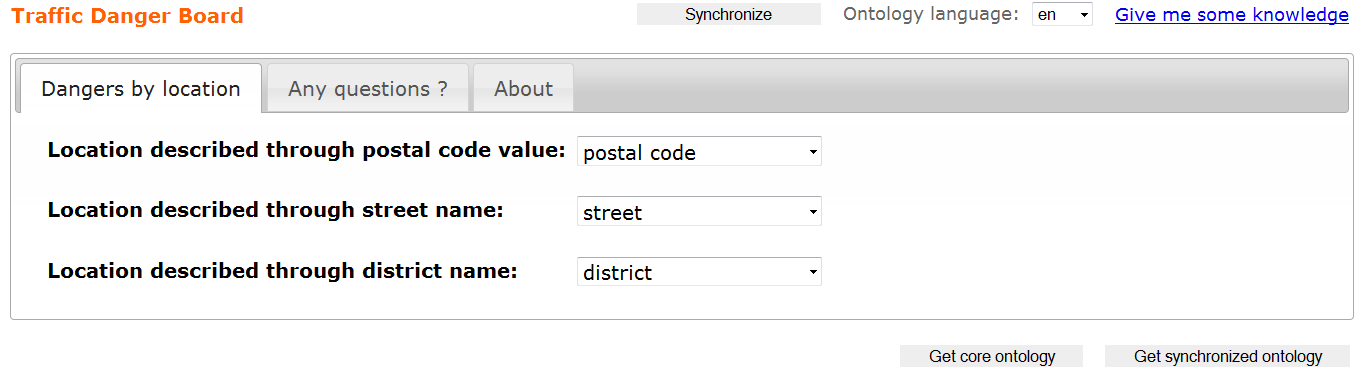
\includegraphics[scale=0.45]{images/chapter4/BoardOverall}
\caption{Overview of the system front page}
\label{fig:boardOverall}
\end{figure}
\vfill
\end{landscape}
}

When this first request to the board page is called, the internal synchronization process is also executed. After the request is completed, we have the possibility of interaction with ontology which is integrated with current traffic conditions data. Such a synchronized ontology is cached in memory. It is why the execution time of first request is longer than further requests. Further requests, connected with refreshing page or invoking reasoner related operations, are very fast, because synchronization process is not being recalled. All system operations are processed on cached ontology. 

\newpage

\noindent If we want to synchronize our ontology with the latest data from database, we have to explicitly invoke synchronization task. It is provided after pushing button called \textit{Synchronize}. That button is located in top right corner of main page, in the toolbar. Top toolbar of the dashboard is shown in Figure \ref{fig:boardTopToolbar}.

\medskip

\begin{figure}[htp]
\centering

\includegraphics[scale=0.6]{images/chapter4/BoardTopToolbar}
\caption{Top toolbar of main page}
\label{fig:boardTopToolbar}
\end{figure}

\noindent In the bottom toolbar (Figure \ref{fig:boardBottomToolbar}), we have the possibility of downloading 2 kinds of ontologies: original (core) and updated (synchronized). It is just a simple feature, which can be helpful for developers or other interested people who want to preview ontology in a raw state - from file, or by loading such a file into an ontology editor such as Protégé.

\medskip

\begin{figure}[htp]
\centering

\includegraphics[scale=0.6]{images/chapter4/BoardBottomToolbar}
\caption{Bottom toolbar of main page}
\label{fig:boardBottomToolbar}
\end{figure}

\noindent Locations data in database are well known. That kind of information is fixed and depends on area we are working with. Based on provided postal codes, we can assign traffic conditions to selected ones (which are further connected to streets and districts). Traffic conditions structure in database is identical as traffic condition subtree structure defined in ontology, which was previously shown in Figure \ref{fig:assertedClassHierarchy}. In Figure \ref{fig:boardMain} we can see core part of the main page.

\medskip

\begin{figure}[htp]
\centering
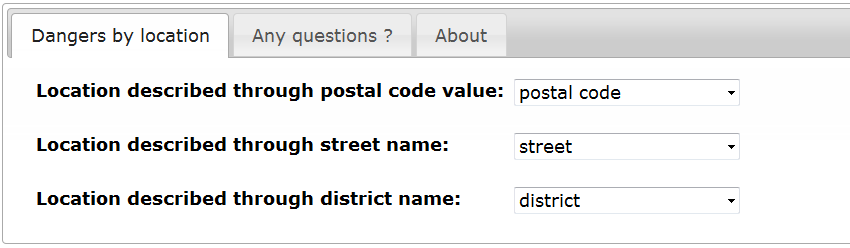
\includegraphics[scale=0.55]{images/chapter4/BoardMain}
\caption{Dangers by location}
\label{fig:boardMain}
\end{figure}

\noindent The main page is divided into 3 tabs. First one, named \textit{Dangers by location}, allows for previewing dangers on desired locations. We can choose dangers connected directly to desired postal code, or indirectly to street or even wider - to district. After choosing desired location, system queries ontology for occurred traffic dangers. Ontology querying means here that system invokes reasoner on cached ontology, and demands answer for question similar to that shown in Section \ref{sub:secondExample}. This time, in the place of \textbf{StareMiasto}, there can be inserted any selected location value. It is shown in Figure \ref{fig:boardMainInferred}.

\newpage

\begin{figure}[htp]
\centering
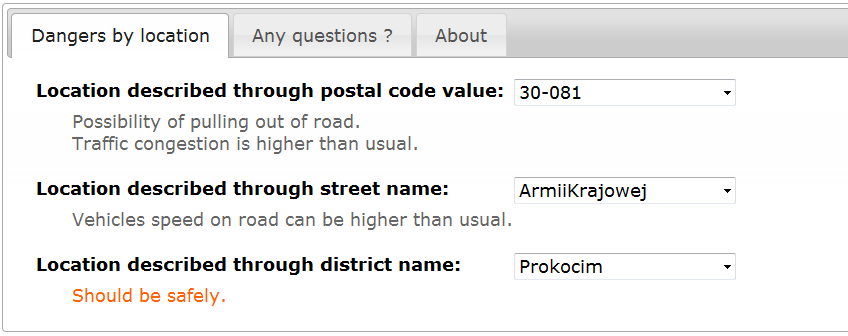
\includegraphics[scale=0.5]{images/chapter4/BoardMainInferred}
\caption{Dangers by location - inferred values}
\label{fig:boardMainInferred}
\end{figure}

\noindent The second tab (called \textit{Any questions?}), shown in Figure \ref{fig:boardQuestions}, displays responses for example predefined questions, our ontology is able to answer.

\afterpage{%
\begin{landscape}
\centering\vspace*{\fill}
\begin{figure}[htp]
\centering
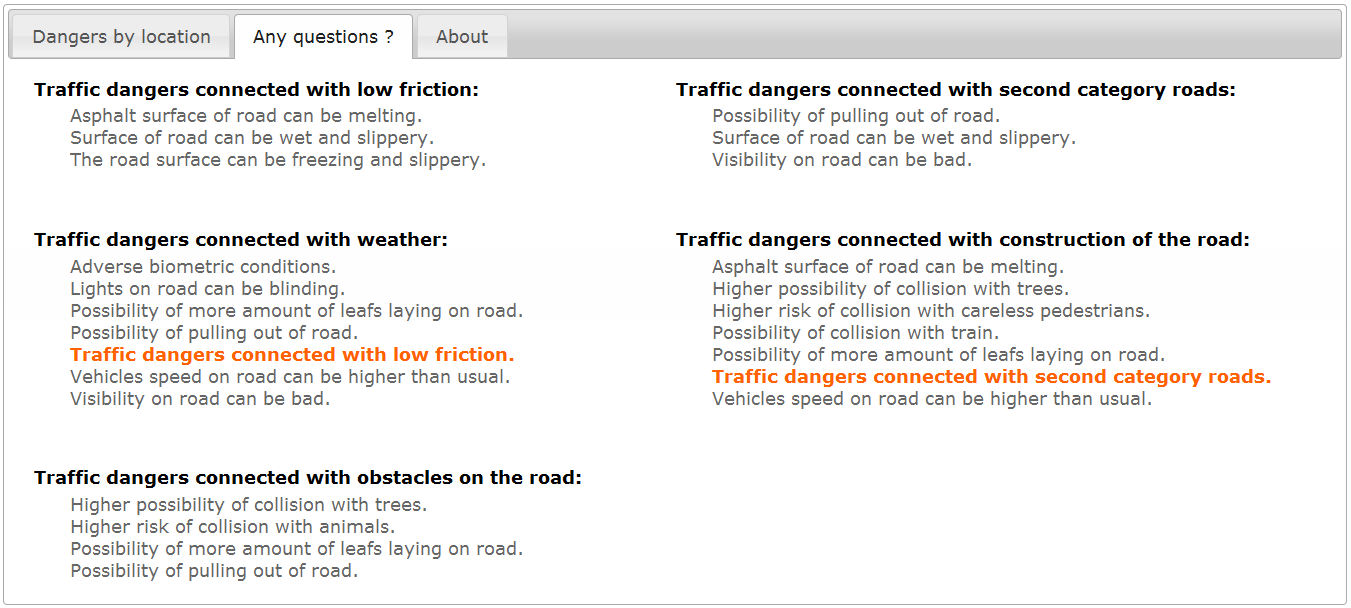
\includegraphics[scale=0.45]{images/chapter4/BoardQuestions}
\caption{Ontology responses for predefined questions}
\label{fig:boardQuestions}
\end{figure}
\vfill
\end{landscape}
}

These questions are not build dynamically on runtime, just like it was always after changing drop down lists values on the previous tab. They are defined statically in the ontology, as defined classes. Defined classes topic was explained earlier in Chapter \ref{cha:trafficDangerOntology}. In the practical shortcut, the reasoner can only automatically classify classes under classes which are defined, because they have fulfilled all necessary and sufficient conditions for reasoning to happen. From the technical point of view, to get answers for such questions, the system has to invoke reasoner on ontology. After that operation, dependencies of all defined classes will be automatically deducted. Developer has to get all that inferred dependent subclasses and provide them to the user. In OWLAPI, the OWL parsing library, that is much easier task to do, than building complex questions dynamically. 

\begin{framed}
\noindent Working with OWLAPI while doing more complex operations, can be a bit confusing for developers, who have never been working with ontologies before. Nevertheless, after review of source code examples provided by the author, library usage will be straightforward. These examples can be found inside trunk branch of the library source code.
\end{framed}

\noindent The last tab on the page, called \textit{About}, provides a brief explanation of the system aim.

\bigskip

\noindent Dashboard provides also the possibility of changing language in which ontology displays data. Traffic danger ontology defines 2 languages: English and Polish. That is the reason why we have only that 2 options provided in drop down list shown on top toolbar (Figure \ref{fig:boardTopToolbar}). Various languages support is provided by the ontology itself. System will data in user preferred language, while fetching data from ontology. Database does not interfere with translations.

When the user choose \textit{Give me some knowledge} hyperlink, located in the right top corner of the dashboard (Figure \ref{fig:boardTopToolbar}), he will be redirected to login page, described in the next section.

\newpage

\subsection{Trusted area authentication form}
\label{sub:trustedAreaAuthenticationForm}

This page provides logging panel (Figure \ref{fig:trustedAreaAuthenticationForm}) for authenticate trusted users, who can modify the database state. 

\medskip

\begin{figure}[htp]
\centering
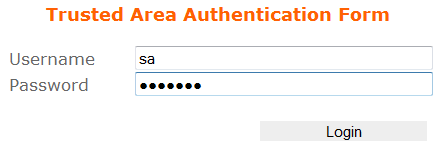
\includegraphics[scale=0.6]{images/chapter4/TrustedAreaAuthenticationForm}
\caption{Logging panel for trusted area}
\label{fig:trustedAreaAuthenticationForm}
\end{figure}

\noindent Database data modification is directly connected with results, users will get while working with ontology, just after synchronization with that updated data. That is the reason of restricted access to control panel. That is be strongly unexpected situation for users, to get inappropriate or even adulterated information about traffic dangers on dedicated areas. This can even provide to potentially unsafe situations on roads, as a result of faulty information about real traffic dangers possibilities. The access is widely restricted but provided for those, who declared inclination for filling database with correct and coherent data.

The database created from scripts, contains example trusted user - username: \texttt{sa}, password: \texttt{traffic}. The user is created only for presentation purposes and should be deleted in production environment. When user provides invalid credentials, appropriate message will be shown on the page.

After login, user will be persisted in the server session. The next entrance to \textit{Traffic Danger Control Panel} will be transparent for user, without necessity of redundant authentication.

\newpage

\subsection{Traffic danger control panel}
\label{sub:trafficDangerControlPanel}

This page allows trusted users for filling current information about specific traffic conditions locations. In the top left corner system displays user, who is actually logged in. The artificially provided user for presentations purposes is called \texttt{sa}:

\medskip

\begin{figure}[htp]
\centering

\includegraphics[scale=0.6]{images/chapter4/PanelTopRight}
\caption{Logged user name}
\label{fig:panelTopRight}
\end{figure}

\noindent Below we can see the base view of the page content:

\medskip

\begin{figure}[htp]
\centering
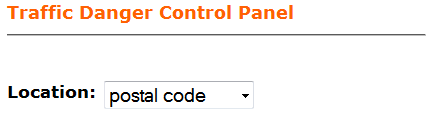
\includegraphics[scale=0.6]{images/chapter4/PanelTopLeft}
\caption{Control panel raw view}
\label{fig:panelTopLeft}
\end{figure}

\noindent After selection of desired postal code value from drop down list, system is building a dynamic tree of traffic conditions. The tree construction is based on database data. Traffic conditions structure in database (provided through table called \texttt{traffic\_condition} shown in Figure \ref{fig:erd} diagram) is identical, as traffic conditions tree structure in ontology, shown in Chapter \ref{cha:trafficDangerOntology} in Figure \ref{fig:assertedClassHierarchy}. ERD diagram of database schema shows, that \texttt{traffic\_conditions} table is connected with \texttt{postal\_code} through intermediate many-to-many relationship table \texttt{traffic\_condition\_2\_postal\_code}. Drop down list is filled with postal codes from database. After selection of desired postal code from the list, system is building current data structure. It is a traffic conditions tree, shown in Figure \ref{fig:panelMain}.

\newpage

\begin{figure}[htp]
\centering
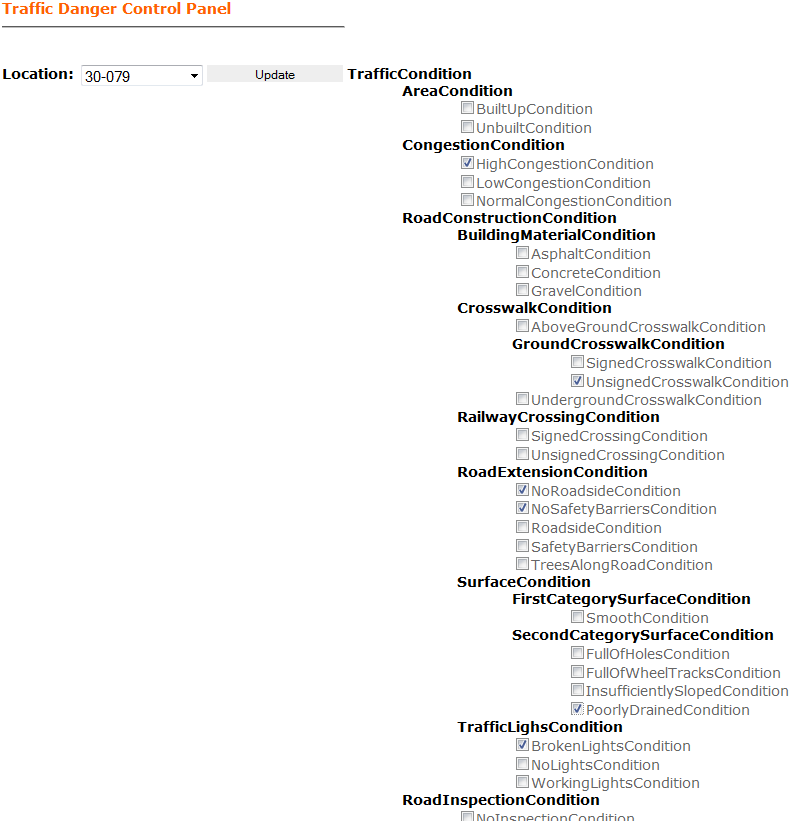
\includegraphics[scale=0.55]{images/chapter4/PanelMain}
\caption{Part of dynamically created view}
\label{fig:panelMain}
\end{figure}

\noindent Users can assign selected location to desired condition by checking radio button next to condition name. When the information is correct, it is ready to be persisted inside database. That is done by pushing \textit{Update} button, next to the drop down list. Knowledge is now updated and can be used for dangers deduction process on front dashboard page, just after the synchronization is done.

\newpage

\section{Technologies inside}
\label{sec:technologiesInside}

\subsection{Introduction}
\label{sub:introductionToTechnologies}

This chapter provides a short preview of main technologies used to build described system. The project is written in Java language in using of Eclipse Java EE IDE. Dependencies management and versioning is the task of Apache Maven tool \cite{MavenHome}.

\subsection{Brief overview}
\label{sub:briefOverview}

\subsubsection{PostgreSQL}
\label{sss:postgreSQL}

Database was designed using latest version of PostgreSQL, which can be downloaded from its home page \cite{PostgresHome}. According to documentation, \textit{"PostgreSQL is an object-relational database management system (ORDBMS) based on  POSTGRES, Version 4.2, developed at the University of California at Berkeley Computer Science Department. POSTGRES pioneered many concepts that only became available in some commercial database systems much later"} \cite{PostgresDocs}.

PostgreSQL is released under the PostgreSQL License, a liberal Open Source license, similar to the BSD or MIT licenses.

\subsubsection{Hibernate}
\label{sss:hibernate}

For interaction with database, system uses object-relational mapping (ORM) library called Hibernate. Hibernate is a library designed for Java language, and provides a framework for mapping an object-oriented domain model to a traditional relational database. Hibernate home page \cite{HibernateHome} provides all necessary information about that technology. There is also a great tutorial \cite{HibernateDocs}, just excellent for learning how to make not only the first steps, but also advanced operations.

One of the most primary features of Hibernate technology, is the possibility of mapping from Java classes to database tables (and from Java data types to SQL data types). Hibernate also provides data query and retrieval facilities. Hibernate automatically generates the SQL calls and relieves the developer from manual result set handling and object conversion, keeping the application portable to all supported SQL databases, with database portability delivered at very little performance overhead.

Hibernate is free software that is distributed under the GNU Lesser General Public License.

\subsubsection{Java Server Pages}
\label{sss:jsp}

According to home page of JavaServer Pages, \textit{"JSP technology enables Web developers and designers to rapidly develop and easily maintain, information-rich, dynamic Web pages that leverage existing business systems. As part of the Java technology family, JSP technology enables rapid development of web-based applications that are platform independent. JSP technology separates the user interface from content generation, enabling designers to change the overall page layout without altering the underlying dynamic content"} \cite{JSPHome}.

JSP technology allows developers to build pages using XML-like tags. Such tags encapsulates the logic that generates the content for the page. The application logic can reside in server-based resources (such as JavaBeans component architecture) that the page accesses with these tags. By separating the page logic from its design and supporting a reusable component-based design, JSP technology to fast and easy build web-based applications. Besides standard markup tags (HTML and XML), JSP uses also scriplet tags for building pages. Scriptlet elements are delimited blocks of Java code which may be intermixed with the markup tags.

JavaServer Pages technology is an extension of the Java Servlet technology. A servlet is a Java class which conforms to the Java Servlet API, a protocol by which a Java class may respond to HTTP requests. Therefore developers may use a servlet to add dynamic content to a web server using the Java platform. JSPs are compiled into servlets by a JSP compiler. The compiler can generate a servlet in Java code that is then compiled by the Java compiler. It can also compile the servlet to byte code which is directly executable. The bytecode must be executed within a Java virtual machine (JVM). It provides an abstract platform-neutral runtime environment. To sum up, servlets are platform-independent, server-side modules extending capabilities of a web server. 

\subsubsection{Spring MVC}
\label{sss:springMVC}

Model View Controller (MVC) is a software architecture which has its roots in Smalltalk \cite{Ree78}. Currently is considered an architectural pattern used in software engineering. 

Applications can contain a mixture of data access code, business logic code, and presentation code. Such applications are difficult to maintain, because interdependencies between all of the components cause strong ripple effects whenever a change is made anywhere. That situation is called as high coupling. Classes depends on so many other classes, that reusing is impossible. Adding new data access code or new data views often requires reimplementing or copping blocks of business logic code, which then requires maintenance in multiple places. The Model View Controller design pattern solves these problems by decoupling data access, business logic, and data presentation and user interaction \cite{SpringMVCSunBlueprints}. The following diagram represents the MVC pattern:

\newpage

\begin{figure}[htp]
\centering
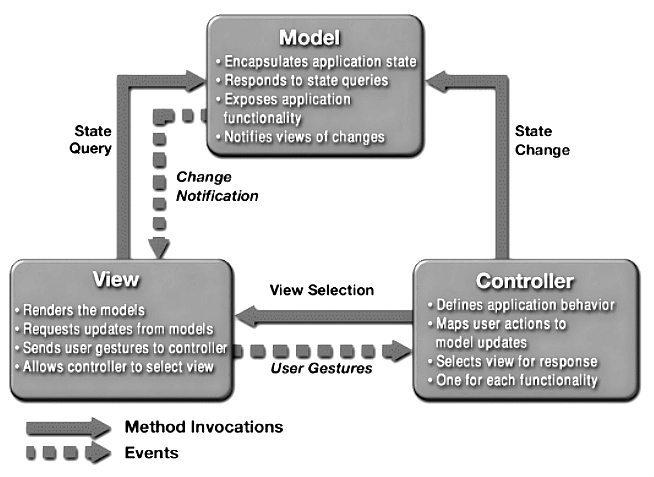
\includegraphics[scale=0.7]{images/chapter4/MVC}
\caption{Model View Controller \cite{SpringMVCSunBlueprints}}
\label{fig:mvc}
\end{figure}

\noindent SpringMVC in one of the implementations of model view controller pattern. It is a part of Spring Framework, an open source application framework for the Java platform. A key design principle in Spring Web MVC and in Spring in general is the \textit{open for extension, closed for modification} principle (OCP principle). Open for extension means, that the behavior of the module can be extended. The module behavior can be changed in new and various ways as the requirements of the application change, or to meet the needs of new applications. Closed for modification means that source code of module designed in this way is inviolate. There is not allowed to make source code changes to it \cite{Mar08}. 

I have used the latest version of SpringMVC, which has a lot of improvements to the previous versions. Simplification in development, part of dynamically evolving Spring Framework application platform and integration with JSP made me choose that technology to build the traffic danger web system. Good source of information about that technology can be found in the documentation on the home page of Spring Framework \cite{SpringHome}.

\subsubsection{jQuery}
\label{sss:jQuery}

According to jQuery home page, \textit{"jQuery is a fast and concise JavaScript Library that simplifies HTML document traversing, event handling, animating, and Ajax interactions for rapid web development. jQuery is designed to change the way that you write JavaScript"} \cite{jQueryHome}.

\newpage

jQuery is a cross-browser JavaScript library designed to simplify the client-side scripting. Cross-browsing refers to the ability for a websites or client-side scripts to support all the web browsers. jQuery's syntax simplifies navigation through the HTML documents, selection of DOM elements, handling events, creating animations and even building Ajax oriented applications in a gentle way. jQuery was released in January 2006 at BarCamp NYC by John Resig. Nowadays the library is used by over 27\% of the 10,000 most visited websites, jQuery is the most popular JavaScript library in use today \cite{jQueryUsageStatistics, UsageOfJavaScriptForWebsites}.

jQuery is free, open source software, under the terms of either the MIT License or the GNU General Public License (GPL) Version 2.

\subsubsection{The OWL API}
\label{sss:theOwlApi}

According to OWL APL home page, \textit{"the OWL API is a Java API and reference implementation for creating, manipulating and serializing OWL Ontologies. The latest version of the API is focused towards OWL 2"} \cite{OWLAPIHome}.

\bigskip

\noindent The OWL API includes the following components:
\begin{itemize}
    \setlength{\itemsep}{0cm}
    \setlength{\parskip}{0cm}

    \item an API for OWL 2 and an efficient in-memory reference implementation,
    \item RDF/XML parser and writer,
    \item OWL/XML parser and writer,
    \item OWL Functional Syntax parser and writer,
    \item Turtle parser and writer,
    \item KRSS parser,
    \item OBO Flat file format parser,
    \item reasoner interfaces for working with reasoners such as FaCT++, HermiT, Pellet and RACER.
\end{itemize}

\noindent The API is closely aligned with the OWL 2 structural specification. It supports parsing and rendering in the syntaxes defined in the W3C specification, namely, the Functional Syntax, RDF/XML, OWL/XML and the Manchester OWL Syntax. Library is written in Java. \textit{"The latest version of the OWL API has been designed to meet the needs of people developing OWL-based applications, OWL editors and OWL reasoners. It is a high level API that is closely aligned with the OWL 2 specification. It includes first class change support, general purpose reasoner interfaces, validators for the various OWL 2 profiles, and support for parsing and serializing ontologies in a variety of syntaxes. The API also has a very flexible design that allows third parties to provide alternative implementations for all major components"} \cite{Hor09}.

The OWL API is open source and is available under the LGPL License.

\subsubsection{HermiT}
\label{sss:hermiT}

According to HermiT home page, \textit{"HermiT is reasoner for ontologies written using the Web Ontology Language (OWL). Given an OWL file, HermiT can determine whether or not the ontology is consistent, identify subsumption relationships between classes, and much more."}

\textit{"HermiT is the first publicly-available OWL reasoner based on a novel "hypertableau" calculus which provides much more efficient reasoning than any previously-known algorithm. Ontologies which previously required minutes or hours to classify can often by classified in seconds by HermiT, and HermiT is the first reasoner able to classify a number of ontologies which had previously proven too complex for any available system to handle. HermiT uses direct semantics and passes all OWL 2 conformance tests for direct semantics reasoners"} \cite{HermiTHome}.

The version (v1.2.3) used in the Traffic Danger Web System is fully compatible with OWLAPI 3.0.0. It is the reason I have chosen that reasoner for working with, because for the time of writing that thesis the Fact++ and Pellet reasoners was not compatible with the newest version of the OWLAPI.

HermiT is open-source and released under LGPL.

\subsubsection{Log4j}
\label{sss:log4j}

Apache Log4j is a Java-based logging utility. It was originally written by Ceki Gülcü and is now a project of the Apache Software Foundation.

\section{Possible directions of development}
\label{sub:possibleDirectionsOfDevelopment}

Future directions of project development can be focused on extensions such as Web Services. Web Services will give the possibility of communication with external systems. That external systems can be perceived as software agents. Their tasks could be focused on periodic connections to our primary system, getting latest information set (serialized into ontology), and creating statistics about traffic dangers. Statistics can visualize frequencies of desired dangers on specific area, classification of safety in desired district at the turn of fixed time, etc.

\section{Summary}
\label{sub:applicationDevelopementSummary}

To summarize, the development of Semantic Web applications with the support of great tool like Protégé, supported by DL reasoner, is quite inspiring development task. Such development process is called as \textit{driven by ontology}. With the support of agile methodologies (like extreme programming) where frequent feedback is crucial for fast and stable system implementation, such development process comes to be powerful. Ontologies can be developed directly by domain experts. Because of direct access to executable systems, charged by recently developed domain models, feedbacks can be made frequently. Best practices from agile methodologies, effective at delivering a particular outcome, can be used in development high-quality domain models. Domain experts may work together with programmers, which can guarantee coherent testing and fast implementation processes.
